\documentclass[12pt, varwidth=15cm]{standalone}

% For large-sized journals the figures should be 84 mm (for double-column text areas), 
% or 174 mm (for single-column text areas) wide and not higher than 234 mm. SAMO


\usepackage[utf8]{inputenc}
\usepackage{bm} % bold math letter
\usepackage{amsmath}
\usepackage{amsfonts}
\usepackage{stanli} % Structure Analisys tikz package
\usepackage{structmech}
\usepackage{siunitx}

% Tikz settings
\usepackage{pgfplots}
\usepackage{tikz}
\usetikzlibrary{decorations.pathreplacing,spy}
\usetikzlibrary{fit}
\usetikzlibrary{shapes.geometric}
\usetikzlibrary{shapes.arrows}
\usetikzlibrary{positioning}
\usetikzlibrary{decorations.pathreplacing,spy}
\usetikzlibrary{arrows.meta}

\pgfdeclarelayer{background}
\pgfsetlayers{background, main}
\pgfplotsset{compat=1.18}

\tikzstyle{decision} = [diamond, aspect=1.8, text centered, fill=white, draw=black, thick]
\tikzstyle{block} = [rectangle, draw=black, thick, fill=white, text centered, rounded corners, minimum height=2em]

\pgfplotsset{
    colormap={coolwarm}{
        rgb255(0cm)=(58,76,192);
        rgb255(1cm)=(64,84,199);
        rgb255(2cm)=(70,93,207);
        rgb255(3cm)=(76,102,214);
        rgb255(4cm)=(82,110,220);
        rgb255(5cm)=(90,120,227);
        rgb255(6cm)=(96,128,232);
        rgb255(7cm)=(103,136,237);
        rgb255(8cm)=(109,144,241);
        rgb255(9cm)=(117,152,246);
        rgb255(10cm)=(124,160,249);
        rgb255(11cm)=(131,166,251);
        rgb255(12cm)=(138,173,253);
        rgb255(13cm)=(145,179,254);
        rgb255(14cm)=(153,186,254);
        rgb255(15cm)=(160,191,254);
        rgb255(16cm)=(167,196,253);
        rgb255(17cm)=(174,201,252);
        rgb255(18cm)=(182,206,249);
        rgb255(19cm)=(188,209,246);
        rgb255(20cm)=(194,212,243);
        rgb255(21cm)=(200,215,239);
        rgb255(22cm)=(206,217,235);
        rgb255(23cm)=(213,219,229);
        rgb255(24cm)=(218,220,223);
        rgb255(25cm)=(223,219,217);
        rgb255(26cm)=(228,216,209);
        rgb255(27cm)=(233,212,201);
        rgb255(28cm)=(237,208,193);
        rgb255(29cm)=(240,204,185);
        rgb255(30cm)=(242,199,178);
        rgb255(31cm)=(244,194,170);
        rgb255(32cm)=(246,187,160);
        rgb255(33cm)=(247,181,152);
        rgb255(34cm)=(247,174,145);
        rgb255(35cm)=(246,167,137);
        rgb255(36cm)=(245,158,127);
        rgb255(37cm)=(243,150,120);
        rgb255(38cm)=(241,142,112);
        rgb255(39cm)=(238,134,105);
        rgb255(40cm)=(234,125,97);
        rgb255(41cm)=(230,114,89);
        rgb255(42cm)=(225,104,82);
        rgb255(43cm)=(220,94,75);
        rgb255(44cm)=(215,84,68);
        rgb255(45cm)=(207,70,61);
        rgb255(46cm)=(201,59,55);
        rgb255(47cm)=(194,45,49);
        rgb255(48cm)=(187,26,43);
        rgb255(49cm)=(179,3,38);
        },
        colormap name=coolwarm, 
        }

        \pgfplotsset{
    colormap={coolwarm_r}{
        rgb255(27cm)=(233,212,201);
        rgb255(28cm)=(237,208,193);
        rgb255(29cm)=(240,204,185);
        rgb255(30cm)=(242,199,178);
        rgb255(31cm)=(244,194,170);
        rgb255(32cm)=(246,187,160);
        rgb255(33cm)=(247,181,152);
        rgb255(34cm)=(247,174,145);
        rgb255(35cm)=(246,167,137);
        rgb255(36cm)=(245,158,127);
        rgb255(37cm)=(243,150,120);
        rgb255(38cm)=(241,142,112);
        rgb255(39cm)=(238,134,105);
        rgb255(40cm)=(234,125,97);
        rgb255(41cm)=(230,114,89);
        rgb255(42cm)=(225,104,82);
        rgb255(43cm)=(220,94,75);
        rgb255(44cm)=(215,84,68);
        rgb255(45cm)=(207,70,61);
        rgb255(46cm)=(201,59,55);
        rgb255(47cm)=(194,45,49);
        rgb255(48cm)=(187,26,43);
        rgb255(49cm)=(179,3,38);
        }
        }

\pgfplotsset{
    colormap={coolwarm_b}{
        rgb255(0cm)=(58,76,192);
        rgb255(1cm)=(64,84,199);
        rgb255(2cm)=(70,93,207);
        rgb255(3cm)=(76,102,214);
        rgb255(4cm)=(82,110,220);
        rgb255(5cm)=(90,120,227);
        rgb255(6cm)=(96,128,232);
        rgb255(7cm)=(103,136,237);
        rgb255(8cm)=(109,144,241);
        rgb255(9cm)=(117,152,246);
        rgb255(10cm)=(124,160,249);
        rgb255(11cm)=(131,166,251);
        rgb255(12cm)=(138,173,253);
        rgb255(13cm)=(145,179,254);
        rgb255(14cm)=(153,186,254);
        rgb255(15cm)=(160,191,254);
        rgb255(16cm)=(167,196,253);
        rgb255(17cm)=(174,201,252);
        rgb255(18cm)=(182,206,249);
        rgb255(19cm)=(188,209,246);
        rgb255(20cm)=(194,212,243);
        rgb255(21cm)=(200,215,239);
        rgb255(22cm)=(206,217,235);
        rgb255(23cm)=(213,219,229);
        rgb255(24cm)=(218,220,223);
        rgb255(25cm)=(223,219,217);
        }
        }
%-----------------------------
%- CUSTOM COLORS
%-----------------------------
\definecolor{accent_b_1}{RGB}{58,76,192}
\definecolor{accent_b_2}{RGB}{103,136,237}
\definecolor{accent_b_3}{RGB}{153,186,254}
\definecolor{accent_b_4}{RGB}{200,215,239}

\definecolor{accent_r_1}{RGB}{179,3,38}
\definecolor{accent_r_2}{RGB}{225,104,82}
\definecolor{accent_r_3}{RGB}{246,167,137}
\definecolor{accent_r_4}{RGB}{237,208,193}

\definecolor{axis_gray}{RGB}{120,120,120}
\definecolor{legend_gray}{RGB}{204,204,204}

%-----------------------------
%- CUSTOM NODES
%-----------------------------
\tikzstyle{point} = [circle,fill=white,draw,inner sep=0pt,minimum size=4pt]
\tikzstyle{forces} = [draw=accent_r_1,-stealth,very thick]
\tikzstyle{lab} = [align=center, fill=white,rounded corners=2pt, inner sep=1pt, font=\footnotesize]
\tikzstyle{arrow_reference} = [-{Triangle[open,length=2.8mm]}, line width=1pt]
%-----------------------------
%- MACROS
%-----------------------------
% Circled letters
\makeatletter
\usetikzlibrary{calc}
\newcommand*\circled[1]{\tikz[baseline=(char.base)]{
    \node[shape=circle, draw, inner sep=0pt, 
        minimum height={\f@size*1.4},] (char) {\vphantom{WAH1g}#1};}}
\makeatother


\newcommand{\norm}[1]{\lVert#1\rVert}
\newcommand{\vect}[1]{\bm{#1}}
\newcommand{\matr}[1]{\bm{#1}}

%-----------------------------
%- STYLE
%-----------------------------

% plot axis styles
\pgfplotsset{general2D/.style={ 
    footnotesize,
    scale only axis,
    axis x line=middle, 
    axis y line=middle, 
    xlabel={$x$}, ylabel={$y$}, 
    axis equal, 
    axis line style={-stealth,semithick},
    } 
}

\pgfplotsset{general3D/.style={ 
    scale only axis, 
    axis line style={-stealth,semithick},
    } 
}

\pgfplotsset{curves/.style={ 
        footnotesize,
        scale only axis, 
        xtick pos=left,
        ytick pos=left,
        axis x line*=bottom, % asterisk = no arrow
        axis y line*=left,
        clip=false,
        enlarge x limits={abs=0.15cm,lower},
        enlarge y limits={abs=0.15cm,lower},
        axis line style={thick, axis_gray, shorten <=0.136cm},
        every axis label/.append style ={axis_gray},
        every tick label/.append style ={axis_gray},
        every x tick/.style={color=axis_gray, thick},
        every y tick/.style={color=axis_gray, thick},
        tick align=outside,
        xlabel near ticks,
        ylabel near ticks,
        legend style={draw=none, font=\scriptsize},
        /pgf/number format/.cd,
        1000 sep={}
    } 
}

\pgfplotsset{curves_left/.style={ 
        scale only axis, 
        xtick pos=left,
        ytick pos=left,
        axis x line*=bottom, % asterisk = no arrow
        axis y line*=left,
        clip=false,
        tick label style={font=\scriptsize},
        every axis label/.append style ={axis_gray, font=\scriptsize},
        every tick label/.append style ={axis_gray},
        every x tick/.style={color=axis_gray, thick},
        every y tick/.style={color=axis_gray, thick},
        enlarge x limits={abs=0.15cm},
        enlarge y limits={abs=0.15cm},
        axis line style={axis_gray,thick, shorten <=0.136cm, shorten >= 0.136cm},
        tick align=outside,
        xlabel near ticks,
        ylabel near ticks,
        legend style={draw=none, font=\scriptsize\color{axis_gray}},
        /pgf/number format/.cd,
        1000 sep={}
    } 
}

\pgfplotsset{curves_right/.style={ 
        scale only axis, 
        xtick pos=left,
        ytick pos=right,
        axis y line*=right,
        x axis line style={draw=none},
        x tick style={draw=none},
        ytick pos=right,
        axis x line*=bottom, % asterisk = no arrow
        axis y line*=left,
        clip=false,
        tick label style={font=\scriptsize},
        every axis label/.append style ={axis_gray, font=\scriptsize},
        every tick label/.append style ={axis_gray},
        every y tick/.style={color=axis_gray, thick},
        enlarge x limits={abs=0.15cm},
        enlarge y limits={abs=0.15cm},
        axis line style={thick, shorten <=0.136cm, shorten >= 0.136cm},
        every y tick/.style={thick},
        tick align=outside,
        ylabel near ticks,
        legend style={draw=none, font=\scriptsize},
        /pgf/number format/.cd,
        1000 sep={}
    } 
}

\pgfplotsset{curves_3D/.style={ 
        footnotesize,
        scale only axis, 
        % xtick pos=left,
        % ytick pos=left,
        % ztick pos=left,
        axis x line*=bottom, % asterisk = no arrow
        axis y line*=left,
        axis z line*=left,
        clip=false,
        % enlarge x limits={abs=0.15cm,lower},
        % enlarge y limits={abs=0.15cm,lower},
        axis line style={thick, axis_gray, shorten <=0.136cm},
        every axis label/.append style ={axis_gray},
        every tick label/.append style ={axis_gray},
        every x tick/.style={color=axis_gray, thick},
        every y tick/.style={color=axis_gray, thick},
        every z tick/.style={color=axis_gray, thick},
        tick align=outside,
        % xlabel near ticks,
        % ylabel near ticks,
        legend style={draw=none, font=\scriptsize},
        /pgf/number format/.cd,
        1000 sep={},
        view={25}{40},
        colormap name=coolwarm,
    } 
}

\pgfplotsset{line_plot/.style={ 
            thick} 
}

\pgfplotsset{scatter_plot_smooth/.style={ 
    thick,
    mark size=1.5, 
    mark=*,
    mark options={solid}, 
    smooth }
}

\pgfplotsset{scatter_plot/.style={ 
    thick,
    mark size=1.5, 
    mark=*,
    mark options={solid}, 
    only marks} 
}

\pgfplotsset{scatter_plot_lin/.style={ 
    thick,
    mark size=1.5, 
    mark=*,
    mark options={solid},} 
}



\begin{document}

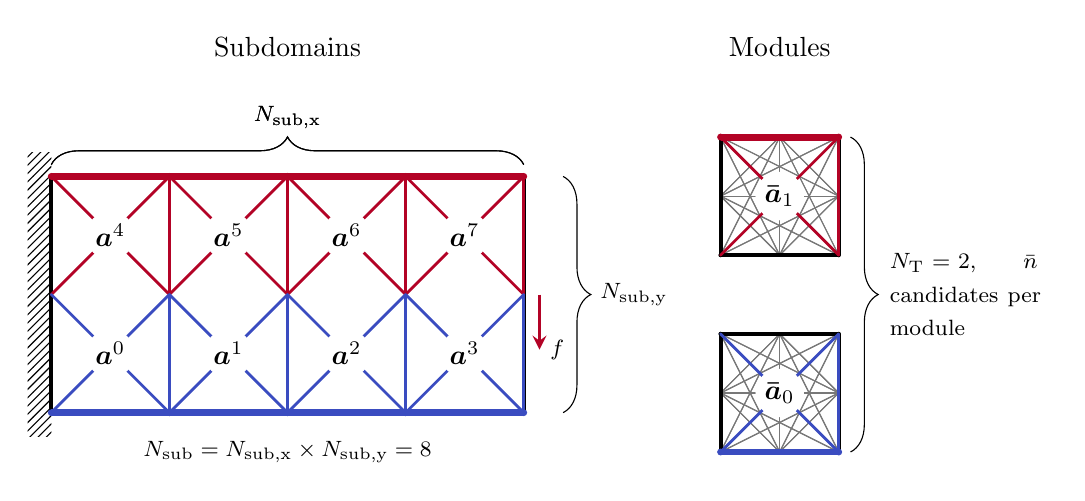
\begin{tikzpicture}

\pgfmathsetmacro\xstep{1.5} % Adjust as needed
\pgfmathsetmacro\ystep{1.5} % Adjust as needed

% % Draw help lines with different step sizes
% \foreach \x in {0,\xstep,...,6} {
%     \foreach \y in {0,\ystep,...,3} {
%         \draw [help lines] (6, \y) -- (0, \y); % Vertical lines
%         \draw [help lines] (\x, 3) -- (\x, 0); % Horizontal lines
%     }
% }

\fill[pattern=north east lines] (-0.3,-0.3) -- (-0.3,3.3) -- (0,3.3) -- (0,-0.3);
    
\point{a}{0}{0};
\point{b}{0}{3};
\point{c}{6}{3};
\point{d}{6}{0};

\beam{2}{a}{b}[1][1];
\beam{2}{b}{c}[1][1];
\beam{2}{c}{d}[1][1];
\beam{2}{d}{a}[1][1];

\begin{scope}[accent_r_1]
    \foreach \x [count=\ii from 0] in {0,\xstep,...,4.5} {
        \draw [line width = 2.5pt] (0+\x,3) -- (1.5+\x,3);
        \draw [line width = 1pt]   (0+\x,1.5) -- (1.5+\x,3);
        \draw [line width = 1pt]   (0+\x,3) -- (1.5+\x,1.5);
        \draw [line width = 1pt]   (1.5+\x,3) -- (1.5+\x,1.5);
        \fill (0+\x,1.5) circle (1pt/2);
        \fill (1.5+\x,1.5) circle (1pt/2);
        \fill (0+\x,3) circle (2.5pt/2);
        \fill (1.5+\x,3) circle (2.5pt/2);
    }
\end{scope}

\begin{scope}[accent_b_1]
    \foreach \x in {0,\xstep,...,4.5} {
        \draw [line width = 2.5pt] (0+\x,0) -- (1.5+\x,0);
        \draw [line width = 1pt]   (0+\x,1.5) -- (1.5+\x,0);
        \draw [line width = 1pt]   (0+\x,0) -- (1.5+\x,1.5);
        \draw [line width = 1pt]   (1.5+\x,0) -- (1.5+\x,1.5);
        \fill (0+\x,1.5) circle (1pt/2);
        \fill (1.5+\x,1.5) circle (1pt/2);
        \fill (0+\x,0) circle (2.5pt/2);
        \fill (1.5+\x,0) circle (2.5pt/2);
    }
\end{scope}

% \begin{scope}[accent_b_1]
%     \draw [line width = 2.5pt] (b2) -- (c2);
%     \draw [line width = 1pt]   (d2) -- (c2);
%     \draw [line width = 1pt]   (b2) -- (d2);
%     \draw [line width = 1pt]   (a2) -- (c2);
%     \fill (a2) circle (1pt/2);
%     \fill (d2) circle (1pt/2);
%     \fill (b2) circle (2.5pt/2);
%     \fill (c2) circle (2.5pt/2);
% \end{scope}

\draw [draw=none]    (0,3.15) -- (6,3.15) node [midway,yshift=1.5cm] {Subdomains};
\node at (9.25,3.15+1.5) {Modules};

    \draw [decorate,decoration={brace,amplitude=10pt},xshift=0pt,yshift=0cm]
    (0,3.15) -- (6,3.15) node [black,midway,yshift=.6cm] {\footnotesize $N_\text{sub,x}$};    

\draw[forces] (6.2,1.5) -- (6.2,1.5-0.7) node[right] {\footnotesize$f$};

\draw [decorate,decoration={brace,amplitude=10pt},xshift=0pt,yshift=0cm]
    (0,3.15) -- (6,3.15) node [black,midway,yshift=.6cm] {\footnotesize $N_\text{sub,x}$};
    
\draw [decorate,decoration={brace,amplitude=10pt},xshift=0cm,yshift=0cm]
    (6.5,3) -- (6.5,0) node [black,midway,xshift=.9cm] {\footnotesize $N_\text{sub,y}$};

\node [black,yshift=-.5cm] at (3,0) {\footnotesize $N_\text{sub}=N_\text{sub,x} \times N_\text{sub,y}=8$};

% \node [black,yshift=-.5cm] at (3,-1) {\footnotesize ${\vect{a}} :=  \{\vect{a}^j \;|\; \forall j \in [1,\dots,N_{\text{sub}}]\}$};

% \node [black,yshift=-.5cm] at (9.25,-1) {\footnotesize {${\bar{\vect{a}}} :=  \{ \bar{\vect{a}}_t \in \mathbb{R}_+^{\bar{n}} \;|\; \forall t \in [1,\dots,N_T]\}$}};

	
% Subdomains

\foreach \xa in {8.5,9.25,10}
            \foreach \ya in {2,2.75,3.5}  
                    \foreach \xx in {8.5,9.25,10}
                        \foreach \yy  in {2,2.75,3.5}  
                                \draw[axis_gray, thin] (\xa, \ya) -- (\xx, \yy);

\foreach \xa in {8.5,9.25,10}
\foreach \ya in {-0.5,0.25,1}  
        \foreach \xx in {8.5,9.25,10}
            \foreach \yy  in {-0.5,0.25,1}  
                    \draw[axis_gray, thin] (\xa, \ya) -- (\xx, \yy);

\point{a1}{0+8.5}{0+2};
\point{b1}{0+8.5}{1.5+2};
\point{c1}{1.5+8.5}{1.5+2};
\point{d1}{1.5+8.5}{0+2};

\beam{2}{a1}{b1}[1][1];
\beam{2}{b1}{c1}[1][1];
\beam{2}{c1}{d1}[1][1];
\beam{2}{d1}{a1}[1][1];
\begin{scope}[accent_r_1]
    \draw [line width = 2.5pt] (b1) -- (c1);
    \draw [line width = 1pt]   (d1) -- (c1);
    \draw [line width = 1pt]   (b1) -- (d1);
    \draw [line width = 1pt]   (a1) -- (c1);
    \fill (a1) circle (1pt/2);
    \fill (d1) circle (1pt/2);
    \fill (b1) circle (2.5pt/2);
    \fill (c1) circle (2.5pt/2);
\end{scope}

\point{b2}{0+8.5}{0-0.5};
\point{a2}{0+8.5}{1.5-0.5};
\point{d2}{1.5+8.5}{1.5-0.5};
\point{c2}{1.5+8.5}{0-0.5};

\beam{2}{a2}{b2}[1][1];
\beam{2}{b2}{c2}[1][1];
\beam{2}{c2}{d2}[1][1];
\beam{2}{d2}{a2}[1][1];

\begin{scope}[accent_b_1]
    \draw [line width = 2.5pt] (b2) -- (c2);
    \draw [line width = 1pt]   (d2) -- (c2);
    \draw [line width = 1pt]   (b2) -- (d2);
    \draw [line width = 1pt]   (a2) -- (c2);
    \fill (a2) circle (1pt/2);
    \fill (d2) circle (1pt/2);
    \fill (b2) circle (2.5pt/2);
    \fill (c2) circle (2.5pt/2);
\end{scope}


\draw [decorate,decoration={brace,amplitude=10pt},xshift=0cm,yshift=0cm]
    (10.15,3.5) -- (10.15,-0.5) node [black,midway,xshift=1.5cm,text width = 2cm] {\footnotesize $N_\text{T}=2$,\quad \quad $\bar{n}$ candidates per module};


        \foreach \x [count=\ii from 0] in {0,\xstep,...,4.5} {
            \filldraw[white,fill=white] (0.75+\x,0.75) circle (0.3); 
            \node[black] at (0.75+\x,0.75) {$\vect{a}^{\ii}$};
        }

        \foreach \x [count=\ii from 4] in {0,\xstep,...,4.5} {
            \filldraw[white,fill=white] (0.75+\x,0.75+1.5) circle (0.3); 
            \node[black] at (0.75+\x,0.75+1.5) {$\vect{a}^{\ii}$};
        }


        \filldraw[white,fill=white] (9.25,0.25) circle (0.3); 
        \node[black] at (9.25,0.25) {$\vect{\bar{a}}_{0}$};
        \filldraw[white,fill=white] (9.25,2.75) circle (0.3); 
            \node[black] at (9.25,2.75) {$\vect{\bar{a}}_{1}$};



	
    
\end{tikzpicture}

\end{document}